\documentclass[a4paper,12pt,titlepage]{article}
\usepackage{amsmath} 
\usepackage{amssymb}
\usepackage[nottoc]{tocbibind}
\usepackage{float}
\usepackage{indentfirst}
\author{\textit{Jiang Yicheng}\\\textit{515370910224}}
\title{\textbf{VV286\\ Honors Mathematics IV\\
Ordinary Differential Equations\\
		Assignment 5}}
\date{\today}
\usepackage{extarrows}
\usepackage{mathrsfs}
\usepackage{dsfont}
\usepackage[top=1 in, bottom=0.8 in, left= 1in, right=1 in]{geometry}
\usepackage{fancyhdr,lastpage}
	\pagestyle{fancy}
	\fancyhf{}
\cfoot{Page \thepage\ of \pageref{LastPage}}
\usepackage{multirow}
\usepackage{gauss}
\usepackage{geometry}
\usepackage{graphicx}
\begin{document}

\maketitle

\section*{Exercise 5.1}
\subsection*{i)}
If $f(x+iy)=u(x,y)+v(x,y)i$ is harmonic, then
\begin{align*}
0&=\Delta f=\dfrac{\partial^2 f}{\partial x^2}+\dfrac{\partial^2 f}{\partial y^2}\\
&=\dfrac{\partial^2 }{\partial x^2}(u+vi)+\dfrac{\partial^2 }{\partial y^2}(u+vi)\\
&=\dfrac{\partial^2 u}{\partial x^2}+i\dfrac{\partial^2 v}{\partial x^2}+\dfrac{\partial^2 u}{\partial y^2}+i\dfrac{\partial^2 v}{\partial y^2}\\
&=\Delta u +i(\Delta v)
\end{align*}

Since $u,v:\Omega\rightarrow \mathbb{R}$, $\Delta u,\Delta v\in\mathbb{R},u,v\in C^2(\mathbb{R})$. So $\Delta u +i(\Delta v)=0\Leftrightarrow \Delta u=0\wedge \Delta v=0$.

So $u,v$ are harmonic.


\subsection*{ii)}
For a function $v$ which satisfies the Cauchy-Riemann differential equations with $u$
\begin{align*}
\Delta f&=\dfrac{\partial^2 u}{\partial x^2}+i\dfrac{\partial^2 v}{\partial x^2}+\dfrac{\partial^2 u}{\partial y^2}+i\dfrac{\partial^2 v}{\partial y^2}\\
&=\dfrac{\partial }{\partial x}\dfrac{\partial v}{\partial y}-i\dfrac{\partial }{\partial x}\dfrac{\partial u}{\partial y} -\dfrac{\partial }{\partial y}\dfrac{\partial v}{\partial x}+i\dfrac{\partial }{\partial y}\dfrac{\partial u}{\partial x}
\end{align*}
Since $u,v$ are potential functions, $\dfrac{\partial }{\partial x}\dfrac{\partial u}{\partial y}=\dfrac{\partial }{\partial y}\dfrac{\partial u}{\partial x},\dfrac{\partial }{\partial x}\dfrac{\partial v}{\partial y}=\dfrac{\partial }{\partial y}\dfrac{\partial v}{\partial x}$. So $f(x+yi)=u(x,y)+iv(x,y)\in C^2(\Omega), \Delta f=0$, i.e. $f$ is harmonic.

According to Cauchy-Riemann differential equations, the harmonic conjugate of $u$ satisfies that 
$$\dfrac{\partial u}{\partial x}=\dfrac{\partial v}{\partial y},\dfrac{\partial u}{\partial y}=-\dfrac{\partial v}{\partial x}$$
Since $u(x,y)=x^3-3xy^2$, 
$$\dfrac{\partial v}{\partial y}=3x^2-3y^2,\dfrac{\partial v}{\partial x}=-(-6xy)=6xy$$
so
$$v=\int6xydx=3x^2y+C(y)$$
where $C(y)$ is a real function of $y$ only. So
$$3x^2-3y^2=\dfrac{\partial v}{\partial y}=3x^2+\dfrac{\partial C(y)}{\partial y}$$
So 
$$\dfrac{\partial C(y)}{\partial y}=-3y^2\Leftrightarrow C(y)=\int -3y^2dy=-y^3+C$$
where $C\in\mathbb{R}$ is a constant.

To sum up, a harmonic conjugate of $u$ is
$$v(x,y)=3x^2y-y^3$$


\section*{Exercise 5.2}
Since $|a|<r<|b|$, series $\sum\limits_{i=0}^{\infty}\Big(\dfrac{a}{z}\Big)^i$ and $\sum\limits_{j=0}^{\infty}\Big(\dfrac{z}{b}\Big)^j$ are convergent and therefore
\begin{align*}
\oint_{\gamma}\dfrac{1}{(z-a)(z-b)}dz&=\oint_{\gamma}\dfrac{1}{bz(1-\dfrac{a}{z})(\dfrac{z}{b}-1)}dz\\
&=-\oint_{\gamma}\dfrac{1}{bz}\sum\limits_{i=0}^{\infty}\Big(\dfrac{a}{z}\Big)^i\cdot \sum\limits_{j=0}^{\infty}\Big(\dfrac{z}{b}\Big)^j dz\\
&=-\oint_{\gamma}\dfrac{1}{bz}\sum\limits_{i=0}^{\infty} \sum\limits_{j=0}^{i}\Big(\dfrac{a}{z}\Big)^j\cdot\Big(\dfrac{z}{b}\Big)^{i-j} dz\\
&=-\sum\limits_{i=0}^{\infty} \sum\limits_{j=0}^{i}a^jb^{j-i-1}\oint_{\gamma}z^{i-2j-1} dz
\end{align*}
Choose parametrization as $\gamma:[0,2\pi)\rightarrow(t),\gamma(t)=re^{it},r>0$, then
 $$\oint_{\gamma}\dfrac{1}{z}dz=\int_0^{2\pi}\dfrac{ire^{it}}{re^{it}}dt=2\pi i$$
$$\forall n\in\mathbb{Z},n\neq -1, \oint_{\gamma}z^n dz=\int_0^{2\pi}ire^{i(n+1)t}dt=\dfrac{1}{n+1}re^{i(n+1)t}|_0^{2\pi}=0$$
So only for $i-2j-1=-1$, i.e. $i=2j$, the integral will not vanish, and therefore
\begin{align*}
\oint_{\gamma}\dfrac{1}{(z-a)(z-b)}dz&=-\sum\limits_{i=0}^{\infty} \sum\limits_{j=0}^{i}a^jb^{j-i-1}\oint_{\gamma}z^{i-2j-1} dz\\
&=-2\pi i\sum\limits_{j=0}^{\infty}a^jb^{-j-1}=-\dfrac{2\pi i}{b}\sum\limits_{j=0}^{\infty}\Big(\dfrac{a}{b}\Big)^j\\
&=-\dfrac{2\pi i}{b}\cdot\dfrac{1}{1-\dfrac{a}{b}}\\
&=\dfrac{2\pi i}{a-b}
\end{align*}

So $\oint_{\gamma}\dfrac{1}{(z-a)(z-b)}dz=\dfrac{2\pi i}{a-b}$.

\section*{Exercise 5.3}
Since $e^{ix^2}$ is holomorphic in an open set containing the $\Gamma _R$, Cauchy's theorem gives
$$\int_0^Re^{ix^2}\,\,dx+\int_0^{\frac{\pi}{4}}e^{i(Re^{it})^2}iRe^{it}dt+\int^0_Re^{i(re^{i\frac{\pi}{4}})^2}r\,\,dr=0$$
and we have
$$\int_0^Re^{i(re^{i\frac{\pi}{4}})^2}e^{i\frac{\pi}{4}}\,\,dr=e^{i\frac{\pi}{4}}\int_0^Re^{-r^2}\,\,dr\xlongequal{t=\sqrt{2}r}\dfrac{1}{2}(1+i)\cdot\dfrac{1}{2}\int_{-\sqrt{2}R}^{\sqrt{2}R}e^{-t^2/2}\,\,dt$$
then let $R\rightarrow\infty$ and we get that
$$\int_0^{\infty}e^{i(re^{i\frac{\pi}{4}})^2}e^{i\frac{\pi}{4}}\,\,dr=\dfrac{1}{4}(1+i)\cdot\sqrt{2\pi}$$

On the other hand, 
\begin{align*}
\Big|\int_0^{\frac{\pi}{4}}e^{i(Re^{it})^2}iRe^{it}dt\Big|&\leqslant R\int_0^{\frac{\pi}{4}}\Big|e^{iR^2(cos(2t)+isin(2t))}\Big|dt=R\int_0^{\frac{\pi}{4}}e^{-R^2sin(2t)}dt\\
&\leqslant R\int_0^{\frac{\pi}{4}}e^{-R^2\frac{2}{\pi}\cdot2t}dt=-\dfrac{\pi R}{4R^2}e^{-R^2\frac{2}{\pi}\cdot2t}\Big|_0^{\frac{\pi}{4}}=-\dfrac{\pi R}{4R^2}(e^{-R^2}-1)\\
&=\dfrac{(1-e^{-R^2})\pi}{4R}\leqslant\dfrac{\pi}{4R}\overset{R\rightarrow\infty}{\longrightarrow}0
\end{align*}
So $$\int_0^{\infty}e^{ix^2}\,\,dx=-\underset{R\rightarrow \infty}{lim}\int_0^{\frac{\pi}{4}}e^{i(Re^{it})^2}iRe^{it}dt+\int_0^{\infty}e^{i(re^{i\frac{\pi}{4}})^2}r\,\,dr=\dfrac{\sqrt{2\pi}}{4}+\dfrac{\sqrt{2\pi}}{4}i$$
So $\int_0^{\infty}sin(x^2)\,\,dx=Im(\int_0^{\infty}e^{ix^2}\,\,dx)=\dfrac{\sqrt{2\pi}}{4},\int_0^{\infty}cos(x^2)\,\,dx=Re(\int_0^{\infty}e^{ix^2}\,\,dx)=\dfrac{\sqrt{2\pi}}{4}$, i.e.
$$\int_0^{\infty}sin(x^2)\,\,dx=\int_0^{\infty}cos(x^2)\,\,dx=\dfrac{\sqrt{2\pi}}{4}$$

\section*{Exercise 5.4}

Since $\dfrac{e^{iz}-1}{2iz}$ is holomorphic in an open set containing the semi circle, Cauchy's theorem gives
$$\int_{-R}^{-\varepsilon}\dfrac{e^{iz}-1}{2iz}\,\,dz+\oint_{-C_{\varepsilon}}\dfrac{e^{iz}-1}{2iz}\,\,dz+\int^{R}_{\varepsilon}\dfrac{e^{iz}-1}{2iz}\,\,dz+\oint_{C_{R}}\dfrac{e^{iz}-1}{2iz}\,\,dz=0$$

Since, 
\begin{align*}
\oint_{C_{R}}\dfrac{e^{iz}-1}{2iz}\,\,dz&= \int_0^{\pi}\dfrac{e^{iRe^{it}}-1}{2iRe^{it}}iRe^{it}dt=\dfrac{1}{2}\int_0^{\pi}e^{iRcost-Rsint}dt-\dfrac{\pi}{2}\\
\Big|\int_0^{\pi}e^{iRcost-Rsint}dt\Big|&\leqslant \int_0^{\frac{\pi}{2}}e^{-R\frac{2}{\pi}\cdot t}dt+\int_{\frac{\pi}{2}}^{\pi}e^{R\frac{2}{\pi}\cdot (t-\pi)}dt\\
&=-\dfrac{\pi}{2R}e^{-R\frac{2}{\pi}\cdot t}\Big|_0^{\frac{\pi}{2}}+\dfrac{\pi}{2Re^{2R}}e^{R\frac{2}{\pi}\cdot t}\Big|^{\pi}_{\frac{\pi}{2}}\\
&=-\dfrac{\pi}{2R}(e^{-R}-1)+\dfrac{\pi}{2Re^{2R}}(e^{2R}-e^R)\\
&=\dfrac{\pi}{2R}(1-e^{-R}+1-e^{-R})\overset{R\rightarrow\infty}{\longrightarrow}0
\end{align*}
So let $R\rightarrow\infty$ and we will obtain
$$\int_{-\infty}^{-\varepsilon}\dfrac{e^{iz}-1}{2iz}\,\,dz+\oint_{-C_{\varepsilon}}\dfrac{e^{iz}-1}{2iz}\,\,dz+\int^{\infty}_{\varepsilon}\dfrac{e^{iz}-1}{2iz}\,\,dz=\dfrac{\pi}{2}$$

Since $\dfrac{e^{iz}-1}{2iz}=\dfrac{1}{2i}\sum\limits_{j=0}^{\infty}\dfrac{1}{(j+1)!}(iz)^j$,
\begin{align*}
&\Big|\oint_{-C_{\varepsilon}}\dfrac{e^{iz}-1}{2iz}\,\,dz\Big|\\
=&\Big|\int^0_{\pi}\dfrac{\sum\limits_{j=1}^{\infty}\dfrac{1}{j!}(i\varepsilon e^{it})^j}{2i\varepsilon e^{it}}\cdot i\varepsilon e^{it}dt\Big|\leqslant\dfrac{1}{2}\int_0^{\pi}\sum\limits_{j=1}^{\infty}\dfrac{1}{j!}|\varepsilon|^jdt\\
=&\dfrac{1}{2}\int_0^{\pi}e^{|\varepsilon|}-1dt=\dfrac{e^{|\varepsilon|}-1}{2}\pi\overset{|\varepsilon|\rightarrow0}{\longrightarrow}0
\end{align*}

So let $\varepsilon\rightarrow0$ and we will obtain
$$\dfrac{\pi}{2}=\int_{-\infty}^{0}\dfrac{e^{iz}-1}{2iz}\,\,dz+\int^{\infty}_{0}\dfrac{e^{iz}-1}{2iz}\,\,dz=\dfrac{1}{2i}\int_{-\infty}^{\infty}\dfrac{cosz}{z}dz+\dfrac{1}{2}\int_{-\infty}^{\infty}\dfrac{sinz}{z}dz-\int_{-\infty}^{\infty}\dfrac{1}{2iz}dz$$
Since $\int_{-\infty}^{\infty}\dfrac{1}{2iz}dz=0$, $\int_{-\infty}^{\infty}\dfrac{sinz}{z}dz=\pi$. Since $\dfrac{sinz}{z}$ is odd, $\int_{-\infty}^{0}\dfrac{sinz}{z}dz=\int_{0}^{\infty}\dfrac{sinz}{z}dz$. So 
$$\int_{0}^{\infty}\dfrac{sinx}{x}dx=\dfrac{\pi}{2}$$


\section*{Exercise 5.5}
\subsection*{i)}
Since $\Big|\dfrac{R^2}{z}\Big|>R$, $\dfrac{f(\zeta)}{\zeta-R^2/\overline{z}}$ is holomorphic function on the disc $D_0$ centered at the origin and of radius $R$, so the integral of $\dfrac{f(\zeta)}{\zeta-R^2/\overline{z}}$ around the circle of radius $R$ 
$$\oint_{C_R} \dfrac{f(\zeta)}{\zeta-R^2/\overline{z}}dz=0$$
i.e.
$$\int_{0}^{2\pi} \dfrac{f(Re^{i\varphi})}{Re^{i\varphi}-R^2/\overline{z}}\cdot iRe^{i\varphi}d\varphi=0$$
According to Cauchy's Integral Formula, $\forall |z|<R$
\begin{align*}
f(z)&=\dfrac{1}{2\pi i}\oint_{C_R} \dfrac{f(\zeta)}{\zeta-z}dz=\dfrac{1}{2\pi i}\int_{0}^{2\pi}\dfrac{f(Re^{i\varphi})}{Re^{i\varphi}-z}\cdot iRe^{i\varphi}d\varphi-\dfrac{1}{2\pi}\int_{0}^{2\pi} \dfrac{f(Re^{i\varphi})Re^{i\varphi}}{Re^{i\varphi}-R^2/\overline{z}} d\varphi\\
&=\dfrac{1}{2\pi}\int_{0}^{2\pi}f(Re^{i\varphi})\Big(\dfrac{Re^{i\varphi}}{Re^{i\varphi}-z}+\dfrac{\overline{z}}{Re^{-i\varphi}-\overline{z}}\Big) d\varphi\\
&=\dfrac{1}{2\pi}\int_{0}^{2\pi}f(Re^{i\varphi})\Big(\dfrac{R^2-|z^2|}{(Re^{i\varphi}-z)(Re^{-i\varphi}-\overline{z})}\Big) d\varphi\\
&=\dfrac{1}{2\pi}\int_{0}^{2\pi}f(Re^{i\varphi})\dfrac{1}{2}\Big(\dfrac{R^2-\overline{z}Re^{i\varphi}+zRe^{i\varphi}-|z|^2+R^2+\overline{z}Re^{i\varphi}-zRe^{i\varphi}-|z|^2|}{(Re^{i\varphi}-z)(Re^{-i\varphi}-\overline{z})}\Big) d\varphi\\
&=\dfrac{1}{2\pi}\int_{0}^{2\pi}f(Re^{i\varphi})\dfrac{1}{2}\Big(\dfrac{Re^{i\varphi}+z}{Re^{i\varphi}-z}+\dfrac{Re^{-i\varphi}+\overline{z}}{Re^{-i\varphi}-\overline{z}}\Big) d\varphi=\dfrac{1}{2\pi}\int_{0}^{2\pi}f(Re^{i\varphi})Re\Big(\dfrac{Re^{i\varphi}+z}{Re^{i\varphi}-z}\Big) d\varphi\\
\end{align*}

To sum up, 
$$f(z)=\dfrac{1}{2\pi}\int_{0}^{2\pi}f(Re^{i\varphi})Re\Big(\dfrac{Re^{i\varphi}+z}{Re^{i\varphi}-z}\Big) d\varphi$$

\subsection*{ii)}
For $z=re^{i\theta}$,
\begin{align*}
&Re\Big(\dfrac{Re^{i\varphi}+z}{Re^{i\varphi}-z}\Big)\\
=&Re\Big(\dfrac{Re^{i\varphi}+re^{i\theta}}{Re^{i\varphi}-re^{i\theta}}\Big)\\
=&Re\Big(\dfrac{(Rcos\varphi+rcos\theta)+i(Rsin\varphi+rsin\theta)}{(Rcos\varphi-rcos\theta)+i(Rsin\varphi-rsin\theta)}\Big)\\
=&Re\Big(\dfrac{((Rcos\varphi+rcos\theta)+i(Rsin\varphi+rsin\theta))((Rcos\varphi-rcos\theta)-i(Rsin\varphi-rsin\theta))}{((Rcos\varphi-rcos\theta)+i(Rsin\varphi-rsin\theta))((Rcos\varphi-rcos\theta)-i(Rsin\varphi-rsin\theta))}\Big)\\
=&\dfrac{(Rcos\varphi+rcos\theta)(Rcos\varphi-rcos\theta)+(Rsin\varphi+rsin\theta)(Rsin\varphi-rsin\theta)}{(Rcos\varphi-rcos\theta)^2+(Rsin\varphi-rsin\theta)^2}\\
=&\dfrac{R^2cos^2\varphi-r^2cos^2\theta+R^2sin^2\varphi-r^2sin^2\theta}{(R^2+r^2-2Rr(cos\varphi cos\theta+sin\varphi sin\theta)}\\
=&\dfrac{R^2-r^2}{R^2-2Rrcos(\theta-\varphi)+r^2}
\end{align*}
So $$Re\Big(\dfrac{Re^{i\varphi}+z}{Re^{i\varphi}-z}\Big)=\dfrac{R^2-r^2}{R^2-2Rrcos(\theta-\varphi)+r^2}$$
for $z=re^{i\theta}$.

\section*{Exercise 5.6}
\subsection*{i)}
Set $f(x+yi):=u(x,y)+iv(x,y)$ where $v(x,y)$ is a harmonic conjugate to the function $u(x,y)$. Then $f$ is holomorphic on the disc centered at the origin and of radius 1. Then for any $0\leqslant r<1,\theta\in\mathbb{R}$
\begin{align*}
&f(rcos\theta+irsin\theta)\\
=&\dfrac{1}{2\pi}\int_{0}^{2\pi}f(e^{i\varphi})Re\Big(\dfrac{e^{i\varphi}+re^{i\theta}}{e^{i\varphi}-re^{i\theta}}\Big) d\varphi\\
=&\dfrac{1}{2\pi}\int_{0}^{2\pi}f(cos\varphi+isin\varphi)\dfrac{1-r^2}{1-2rcos(\theta-\varphi)+r^2} d\varphi\\
=&\dfrac{1}{2\pi}\int_{0}^{2\pi}P_r(\theta-\varphi)u(cos\varphi,sin\varphi) d\varphi+\dfrac{i}{2\pi}\int_{0}^{2\pi}P_r(\theta-\varphi)v(cos\varphi,sin\varphi) d\varphi
\end{align*}
where $P_r(\theta-\varphi)=\dfrac{1-r^2}{1-2rcos(\theta-\varphi)+r^2}$. Since $u,v$ are real valued functions, 
$$u(rcos\theta,rsin\theta)=\dfrac{1}{2\pi}\int_{0}^{2\pi}P_r(\theta-\varphi)u(cos\varphi,sin\varphi) d\varphi$$

\subsection*{ii)}
For $r=1$, it's the solution to the \textit{Dirichlet problem}. Also from $i)$ we can know that 
$u(rcos\theta,rsin\theta)=\dfrac{1}{2\pi}\int_{0}^{2\pi}P_r(\theta-\varphi)u(cos\varphi,sin\varphi) d\varphi=\dfrac{1}{2\pi}\int_{0}^{2\pi}P_r(\theta-\varphi)f(cos\varphi,sin\varphi) d\varphi$ for $r<1$.
\begin{align*}
&\Delta u(x,y)\\=&\Delta_{r,\theta}u(r,\theta)=\dfrac{1}{r^2}\dfrac{\partial^2 u}{\partial \theta^2}+\dfrac{1}{r}\dfrac{\partial u}{\partial r}+\dfrac{\partial^2 u}{\partial r^2}\\
=&\dfrac{1}{r^2}\dfrac{\partial^2 }{\partial \theta^2}\dfrac{1}{2\pi}\int_{0}^{2\pi}f(cos\varphi+isin\varphi)\dfrac{1-r^2}{1-2rcos(\theta-\varphi)+r^2} d\varphi\\
&+\dfrac{1}{r}\dfrac{\partial }{\partial r}\dfrac{1}{2\pi}\int_{0}^{2\pi}f(cos\varphi+isin\varphi)\dfrac{1-r^2}{1-2rcos(\theta-\varphi)+r^2} d\varphi\\
&+\dfrac{\partial^2 }{\partial r^2}\dfrac{1}{2\pi}\int_{0}^{2\pi}f(cos\varphi+isin\varphi)\dfrac{1-r^2}{1-2rcos(\theta-\varphi)+r^2} d\varphi\\
=&\dfrac{1}{r^2}\dfrac{1}{2\pi}\int_{0}^{2\pi}f(cos\varphi+isin\varphi)2r(1-r^2)\dfrac{4r(1+r^2)-(1+10r^2+r^4)cos(\theta-\varphi)+4r^2cos^3(\theta-\varphi)}{(1-2rcos(\theta-\varphi)+r^2)^4} d\varphi\\
&+\dfrac{1}{r}\dfrac{1}{2\pi}\int_{0}^{2\pi}f(cos\varphi+isin\varphi)\dfrac{-4r+2(1+r^2)cos(\theta-\varphi)}{(1-2rcos(\theta-\varphi)+r^2)^2} d\varphi\\
&+\dfrac{1}{2\pi}\int_{0}^{2\pi}f(cos\varphi+isin\varphi)\\&\dfrac{(12r^4+8r^2-4)+(-4r^5-40r^3-4r)cos(\theta-\varphi)+(8r^4+32r^2+8)cos^2(\theta-\varphi)-16rcos^3(\theta-\varphi)}{(1-2rcos(\theta-\varphi)+r^2)^4} d\varphi\\
&=0
\end{align*}

So $u$ is harmonic and therefore it's a solution to the Dirichlet problem for the unit disc.





\section*{Exercise 5.7}
For $r<1$,
\begin{align*}
&u(r,\theta)\\
=&\dfrac{1}{2\pi}\int_{-\pi}^{\pi}P_r(\theta-\varphi)u(1,\varphi)d\varphi\\
=&-\dfrac{1}{2\pi}\int_{-\pi}^{0}\dfrac{1-r^2}{1-2rcos(\theta-\varphi)+r^2}d\varphi+\dfrac{1}{2\pi}\int_{0}^{\pi}\dfrac{1-r^2}{1-2rcos(\theta-\varphi)+r^2}d\varphi\\
=&-\dfrac{1}{\pi}arctan\Big(\dfrac{1+r}{1-r}tan\dfrac{\varphi-\theta}{2}\Big)\Big|^0_{-\pi}+\dfrac{1}{\pi}arctan\Big(\dfrac{1+r}{1-r}tan\dfrac{\varphi-\theta}{2}\Big)\Big|_0^{\pi}\\
=&\dfrac{1}{\pi}arctan\Big(\dfrac{1+r}{1-r}tan\dfrac{\theta}{2}\Big)-\dfrac{1}{\pi}arctan\Big(\dfrac{1+r}{1-r}cot\dfrac{\theta}{2}\Big)+\dfrac{1}{\pi}arctan\Big(\dfrac{1+r}{1-r}tan\dfrac{\theta}{2}\Big)\\
&+\dfrac{1}{\pi}arctan\Big(\dfrac{1+r}{1-r}cot\dfrac{\theta}{2}\Big)\\
=&\dfrac{2}{\pi}arctan\Big(\dfrac{1+r}{1-r}tan\dfrac{\theta}{2}\Big)
\end{align*}
So
$$u(r,\theta)=\left\{
\begin{aligned}
&\dfrac{2}{\pi}arctan\Big(\dfrac{1+r}{1-r}tan\dfrac{\theta}{2}\Big),0\leqslant r<1\\
&-1\,\,\,\,\,\,\,\,\,\,\,\,\,\,\,\,\,\,\,\,\,\,\,\,\,\,\,\,\,\,\,\,\,\,\,\,\,\,\,\,\,\,\,\,\,\,,r=1\wedge -\pi\leqslant\theta<0\\
&1\,\,\,\,\,\,\,\,\,\,\,\,\,\,\,\,\,\,\,\,\,\,\,\,\,\,\,\,\,\,\,\,\,\,\,\,\,\,\,\,\,\,\,\,\,\,\,\,\,\,\,\,\,,r=1\wedge 0\leqslant\theta<\pi\\
\end{aligned}
\right.
$$
\begin{figure}[H]
    \centering
    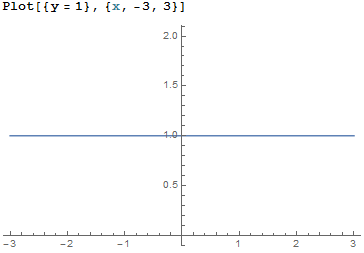
\includegraphics[scale=1]{1.png}
    \caption{The figure of the solution to the Dirichlet problem}

\end{figure}



$\mathbf{N}$
\end{document}
